\chapter{Path Integrals for Interacting Real Scalar Fields}

We incorporate interactions to our theories by adding terms to the Hamiltonian as perturbations. In this case, the path integral will require a series expansion, for which \textit{Feynman diagrams} will be a useful tool for graphically representing, organizing and enumerating terms.
\section{Perturbative treatment of gaussian integrals}
To introduce the core idea behind Feynman Diagrams, we consider a simpler problem, a ``baby problem" in which diagrams can be used to represent terms of a series. Inpired by Zee's \cite{zee2010quantum} approach, we consider the problem of evaluating the integral
\begin{equation}
    Z(J)=\int\dd q\, \exp[-\frac{1}{2}m^2q^2+\frac{1}{3!}gq^3+Jq],
    \label{z_toy}
\end{equation}
where $m$, $g$ and $J$ hold no functional dependence with $q$. We separate the linear and quadratic terms inside the exponential from the cubic term and expand the exponential with the cubic term:
\begin{equation}
      Z(J)=\int\dd q\, e^{-\frac{1}{2}m^2q^2+Jq}\qty[1+\frac{1}{3!}gq^3+\frac{1}{2!(3!)^2}g^2q^6+\frac{1}{3!(3!)^3}g^3q^9+\dots].
\end{equation}
We highlight the result:
\begin{equation}
    \int\dd q\, q^{n}e^{-\frac{1}{2}m^2q^2+Jq}=\qty(\dv{J})^{n}\int\dd q\,e^{-\frac{1}{2}m^2q^2+Jq}
\end{equation}
which is valid for even and odd $n$, although the odd powers yield a null integral (odd functions in symmetric interval). Then $Z(J)$ reads
\begin{equation}
\begin{aligned}
      Z=&\int\dd q\, e^{-\frac{1}{2}m^2q^2+Jq}\qty[1+\frac{1}{3!}gq^3+\frac{1}{2!(3!)^2}g^2q^6+\frac{1}{3!(3!)^3}g^3q^9+\dots]\\
      =&\qty[1+\frac{1}{3!}g\qty(\dv{J})^3+\frac{1}{2!(3!)^2}g^2\qty(\dv{J})^6+\frac{1}{3!(3!)^3}g^3\qty(\dv{J})^9+\dots]\int\dd q\, e^{-\frac{1}{2}m^2q^2+Jq}\\
      =&\exp[\frac{1}{3!}\,g\qty(\dv{J})^3]\int\dd q\, e^{-\frac{1}{2}m^2q^2+Jq}.
\end{aligned}      
\label{interac_out}
\end{equation}
Completing the square we evaluate the Gaussian integral
\begin{equation}
    \int\dd q\, e^{-\frac{1}{2}m^2q^2+Jq}=\sqrt{\frac{2\pi}{m^2}}\,e^{J^2/2m^2},
\end{equation}
so that
\begin{equation}
    Z(J)=\sqrt{\frac{2\pi}{m^2}}\exp[\frac{1}{3!}\,g\qty(\dv{J})^3]\exp[\frac{J^2}{2m^2}].
    \label{Z_exps}
\end{equation}
Up to a normalization constant, we have the series
\begin{equation}
    Z(J)\propto\sum_{V=0}^\infty\frac{1}{V!}\qty[\frac{1}{3!}\,g\qty(\dv{J})^3]^V\sum_{P=0}^\infty\frac{1}{P!}\qty[\frac{J^2}{2m^2}]^P.
    \label{Z_series}
\end{equation}
To organize its terms we will associate to each term a graph. The task of evaluating the series up to a certain order will be simplified: we only need to draw diagrams corresponding to that order and translate to the desired term in the series. To see how this can be done, consider, more explicitly, expansion (\ref{Z_series}):
\begin{equation}
\begin{aligned}
    Z(J)=&\qty[1+\frac{1}{3!}g\qty(\dv{J})^3+\frac{1}{2!(3!)^2}g^2\qty(\dv{J})^6+\frac{1}{3!(3!)^3}g^3\qty(\dv{J})^9+\dots]\times\\
    &\qty[1+\frac{J^2}{2m^2}+\frac{1}{2!}\qty(\frac{J^2}{2m^2})^2+\frac{1}{3!}\qty(\frac{J^2}{2m^2})^3+\frac{1}{4!}\qty(\frac{J^2}{2m^2})^4+\dots].
    \label{expansaozona}
\end{aligned}
\end{equation}
Suppose we are interested in the term linear in $g$ and cubic in $J$. This corresponds to the term resulting from the product of the second term in the first pair of brackets by the fourth term in the second pair, that is:
    \begin{equation}
    \frac{1}{3!}g\qty(\dv{J})^3\times\frac{1}{3!}\qty(\frac{J^2}{2m^2})^3=\qty(\frac{1}{2m^2})^3\frac{6!}{(3!)^3}gJ^3.
    \label{termogJ3}
    \end{equation}
Next, we draw a diagram
consisting of lines, blobs and vertices that must join three lines (for this problem):
\begin{itemize}
    \item A line corresponds to a factor of $\qty(\frac{1}{m^2})$: the ``propagator" for this theory;
    \item A vertex corresponds to a factor $g$;
    \item Blobs at the end of lines should correspond to factors $J$: the sources
\end{itemize}
 A diagram for term (\ref{termogJ3}), for instance, needs three sources, three lines and one vertex, as indicated by Figure \ref{tres}.
 \begin{figure}[h]
 \centering
     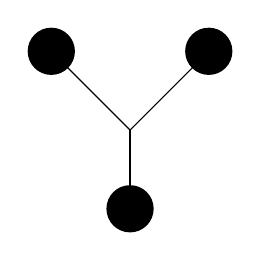
\begin{tikzpicture}
                 \fill[black] (1,1) circle (0.3 cm);
                 \fill[black] (-1,1) circle (0.3 cm);
                 \fill[black] (0,-1) circle (0.3 cm);
                 \draw (0,0) -- (1,1);
                 \draw (0,0) -- (-1,1);
                 \draw (0,0) -- (0,-1);
            \end{tikzpicture}
    \caption{Diagram for term (\ref{termogJ3}) of (\ref{Z_series}).}
    \label{tres}
\end{figure}\\

The number of sources and vertices in a diagram determine the order in $J$ and $g$ of the term in (\ref{Z_series}) that the graph represents.
To reconstruct a term from a diagram, we identify each element in the graph (lines, vertices, blobs), and associate to them the corresponding factor ($m^{-2}$, $g$ and $J$). The complete term is the multiplication of all the factors present in a diagram. As another example, the term linear both in $g$ and $J$ is
\begin{equation}
    \frac{1}{3!}g\qty(\dv{J})^3\times\frac{1}{2!}\qty(\frac{J^2}{2m^2})^2=\qty(\frac{1}{2m^2})^2\frac{4!}{2!}\frac{1}{3!}gJ,
    \label{termogJ}
\end{equation}
resulting from the product of the second term on the first bracket by the third term on the second one in (\ref{expansaozona}). A diagram for this term has one vertex, two propagators, and one source. As vertices must join three lines, one of the propagators must be in a \textit{loop}, as shown by Figure \ref{gJ}.
\begin{figure}[h]
    \centering
    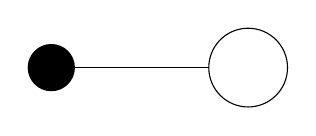
\begin{tikzpicture}
     \fill [black] (0,0) circle (0.3 cm);
    \draw (0,0) -- (2,0);
    \draw (2.5,0) circle (0.5 cm);
    \end{tikzpicture}
    \caption{Diagram for term (\ref{termogJ}) of (\ref{Z_series}) and for term (\ref{gJ_phi3}) of (\ref{Z_1})}
    \label{gJ}
\end{figure}

\section{Feynman diagrams for $\phi^3$ theory}
Integral (\ref{z_toy}) can be regarded as the path integral for a field theory in a single space  dimension (1+1).  Now we consider the usual 3+1 dimensions real scalar field theory. The interaction Lagrangian we will consider is $\mathcal{L}_1=\frac{1}{3!}g\phi^3$, which gives the so-called \textit{phi-cubed} theory. We assume the conditions we required for the validity of the LSZ formula are met, that is
\begin{equation}
 \vev{\phi(x)}=0\quad,\quad \bra{k}{\phi(x)}\ket{0}=e^{-ikx} 
\end{equation}
with one-particle states normalization
\begin{equation}
    \braket{k^\prime}{k}=(2\pi)^32k^0\delta^3(\vb{k}-\vb{k}^\prime).
\end{equation}
To satisfy these, the field can be scaled and shifted, resulting in the Lagrangian
\begin{equation}
    \mathcal{L}=-\frac{1}{2}Z_\phi\partial_\mu\phi\partial^\mu\phi-\frac{1}{2}Z_mm^2\phi^2+\frac{1}{3!}Z_gg\phi^3+Y\phi.
\end{equation}
The functional integral reads
\begin{equation}
    Z(J)=\braket{0}_J=\int\mathcal{D}\phi\,\exp[i\int\dd^4 x\,(\mathcal{L}_0(\phi,\partial_\mu\phi)+\mathcal{L}_1(\phi)+J(x)\phi)]
    \label{path_integral_interacting}
\end{equation}
where we split the Lagrangian as 
\begin{equation}
    \mathcal{L}_0=-\frac{1}{2}\partial_\mu\phi\partial^\mu\phi-\frac{1}{2}m^2\phi^2
    \label{L_0}
\end{equation}
\begin{equation}
    \mathcal{L}_1=\frac{1}{3!}Z_g g \phi^3 + \mathcal{L}_{\text{ct}}
\end{equation}
\begin{equation}
    \mathcal{L}_{\text{ct}}=-\frac{1}{2}(Z_\phi -1)\partial_\mu\phi\partial^\mu\phi-\frac{1}{2}(Z_m-1)m^2\phi^2+Y\phi
    \label{L_ct}
\end{equation}
in order to take advantage of the same procedure we did in (\ref{interac_out}) and our knowledge of the free theory path integral. $\mathcal{L}_{\text{ct}}$ stands for ``counterterm" Lagrangian. As in (\ref{interac_out}), we have
\begin{equation}
    Z(J)=\exp[i\int\dd^4x\,\mathcal{L}_1\qty(\frac{1}{i}\fdv{J(x)})]\int\mathcal{D}\phi\, \exp[i\int\dd^4 x\,(\mathcal{L}_0+J\phi)]
    \label{interac_out_functional}
\end{equation}
where, as we have seen in previous work
\begin{equation}
    Z_0=\int\mathcal{D}\phi\, \exp[i\int\dd^4 x\,(\mathcal{L}_0+J\phi)]=\exp[\frac{i}{2}\int\dd^4x\,\dd^4x^\prime\,J(x)\Delta(x-x^\prime)J(x^\prime)].
\end{equation}

We proceed to calculate (\ref{path_integral_interacting}) ignoring, for now, the counterterms, that is, with interaction Lagrangian being $\mathcal{L}_1=\frac{Z_gg}{3!}\phi^3(x)$ solely. We call this portion of the integral $Z_1$.
\begin{equation}
\begin{aligned}
      Z_1(J)&\propto\exp[\frac{iZ_gg}{3!}\int\dd^4x\,\qty(\frac{1}{i}\fdv{J(x)})^3]Z_0(J)\\
      &=\sum_{V=0}^\infty\frac{1}{V!}\qty[\frac{iZ_gg}{3!}\int\dd^4x\,\qty(\frac{1}{i}\fdv{J(x)})^3]^V\\&\times\sum_{P=0}^{\infty}\frac{1}{P!}\qty[\frac{i}{2}\int\dd^4x\,\dd^4x^\prime\,J(x)\Delta(x-x^\prime)J(x^\prime)]^P,
      \label{Z_1}
\end{aligned}
\end{equation}
which are analogous to (\ref{Z_exps}) and (\ref{Z_series}). Note we have a  proportionality rather than an equality since the $\epsilon$ trick \footnote{Recall we are considering $\mathcal{H}\to(1-i\epsilon)\mathcal{H}$} does not preserve normalization, which will be imposed by hand. Acting with the functional derivatives leaves $E=2P-3V$ sources remaining, and an overall phase of $i^{P-2V}=i^{V+E-P}$ in (\ref{Z_1}). For fixed $V$ and $P$, we have $3V$ functional derivatives acting in $2P$ sources, so there are $(2P)!/(2P-3V)!$ combinations for such arrangements. \\

To enumerate and reconstruct a term from (\ref{Z_1}) we introduce \textit{Feynman diagrams}, in a similar manner we did for our simpler example of last section. We associate:
\begin{itemize}
    \item a propagator $\frac{1}{i}\Delta(x-y)$ to a line connecting points $x$ and $y$;
    \item a source $i\int\dd^4 x\,J(x)$ to a blob at the end or beginning of a line;
    \item an amplitude $iZ_gg\int\dd^4x$ to a vertex joining three lines.
\end{itemize}

To get a sense of what we are doing when constructing these diagrams, we will calculate one term and build its corresponding diagram. We consider a diagram with one vertex and two propagators, that is, the term with $V=1$ and $P=2$ in (\ref{Z_1}), giving $E=2P-3V=1$ \textit{externals}, the remaining number of sources. Our task then is to expand 
\begin{equation}
    \frac{iZ_g g}{2!3!}\int\dd^4x\qty(\frac{1}{i}\fdv{J(x)})^3\qty[\frac{i}{2}\int\dd^4y\,\dd^4zJ(y)\Delta(y-z)J(z)]^2.
    \label{expanding_term}
\end{equation}
A laborious task which goes like this
%Tinha feito umas simplificações e a conta saiu com essas terminologias diferentes, vou arrumar. $\delta_x= \fdv{J(x)}$, $J_y=J(y)$ and $\Delta_{yz}=\Delta(y-z)$
\begin{equation}
    \begin{aligned}
          & = \frac{Z_g g}{2^22!3!}\int\dd^4x\, \qty(\fdv{J(x)})^3\int\dd^4y\,\dd^4z\,\dd^4w\,\dd^4 v J(y)\Delta(y-z)J(z)J(w)\Delta(w-v)J(v)\\
         &\vdots\\ &=\frac{Z_gg}{48}\int\dd^4x\,\dd^4y\,\dd^4z\,\dd^4w\,\dd^4v \Big[\delta^4(y-x)\Delta(y-z)\delta^4(z-x)\delta^4(w-x)\Delta(w-v)J(v)\\
         &\qquad+\delta^4(y-x)\Delta(y-z)\delta^4(z-x)J(w)\Delta(w-v)\delta^4(v-x)+\overbrace{\dots}^{\text{22 terms}}\Big]\\
         &=\frac{Z_gg}{48} \qty[\int\dd^4x\,\dd^4v\Delta(0)\Delta(x-v)J(v)+\int\dd^4x\,\dd^4w\,\Delta(0)J(w)\Delta(w-x)+\overbrace{\dots}^{\text{22 terms}}]
    \end{aligned}
\end{equation}
In the second equality, the other $22$ terms are  just like the ones indicated: all of them consist of three Delta functions, two propagators and one source, but with variables at which these objects are evaluated permuted. In the last line, integration simplify the Deltas in each term, and since the resulting 24 terms differ only by the dummy integration variables, we find
\begin{equation}
    \frac{Z_gg}{2} \int\dd^4x\,\dd^4v\Delta(0)\Delta(x-v)J(v)
    \label{gJ_phi3}.
\end{equation}
This term can be found from the following diagram: $\frac{1}{i}\Delta(0)$ corresponds to a propagator taking a point into itself: a loop. $\frac{1}{i}\Delta(x-y)$ corresponds to a line from $x$ to $y$ and a vertex accounts for $iZ_gg\int\dd^4x$, connecting three lines. We also need a source, which is attached to the free end of the $\Delta(x-y)$. The diagram is assembled as we connect the two ends of $\Delta(0)$ to $\Delta(x-y)$ propagator, being identical to diagram presented in Figure \ref{gJ}.\\

We see that the diagram accounts for everything except for the $1/2$ factor. We now focus on how to determine the numerical factors accompanying a term cast from a diagram. This is the problem of determining how many diagrams correspond to the same term in (\ref{Z_1}). To assess this issue, we note that in the first series of (\ref{Z_1}) (the one summing over $V$), for a given fixed $V$, we can rearrange the order of the three functional derivatives and the order of the $V$ vertices. The swap of derivatives (which effectively swaps the ends of propagators) gives $3!$ different diagrams per vertex, and the swap of vertices gives $V!$ different diagrams. This accounts for $(3!)^VV!$ diagrams to the same term, since these changes leave the diagram invariant. Similarly, in the second series (the one summing over $P$), we can rearrange the two sources and also the $P$ propagators themselves, so there are $(2!)^PP!$ diagrams for the same term. All these factors combined cancel the $((3!)^VV!(2!)^PP!)^{-1}$ factor in (\ref{Z_1}). \\
%some of these multiple rearrangements of sources and propagators give the same diagram then we have overcounted terms and the factors will not exactly cancel,

However, this reasoning can lead to an overcount in some situations. Sometimes the factors don't exactly cancel, just as in our example above (\ref{gJ_phi3}), where we got a $1/2$ left. The overcount in our enumeration considerations is related to some \textit{symmetry} property of a diagram.
%happening whenever rearrangement of propagators gives the same diagram as a rearrangement of sources. 
We must identify how much we have overcounted, so we can divide each term in the series by its corresponding diagram's \textit{symmetry factor}.
%We must be able to identify how many of these terms giving equivalent diagrams there are so we can divide each term in the series by its corresponding diagram's \textit{symmetry factor}, which indicates how much we overcounted that specific term.\\
If we take a look at diagram of Figure (\ref{gJ}) we see that swapping the ends of the loop is equivalent to swapping two legs of the vertex. So there are actually two diagrams corresponding to the same term, thus justifying the $1/2$ factor.\\

Diagram in Figure (\ref{tres}) can also represent a term in (\ref{Z_1}):
 \begin{equation}
     \frac{iZ_g g}{ 3!}\int\dd^4x\,\dd^4y\,\dd^4z\,\dd^4w\, J(y)\Delta(y-x)J(z)\Delta(z-x)J(w)\Delta(w-x).
 \end{equation}
 We have three propagators and any of the $3!$ rearrangements of them gives us the same diagram. This justifies the symmetry factor. Other examples of diagrams are the ones indicated in Figure (\ref{p3v2e0}), with their corresponding symmetry factor. We also highlight an important diagram we will need when dealing with scattering, which that of Figure (\ref{tree_diagramJ}). A complete list of diagrams in $\phi^3$ theory can be found in Chapter 9 of Srednicki \cite{srednicki2007quantum}.\\
 \begin{figure}[h]
    \begin{subfigure}[b]{0.45\textwidth}
    \centering
    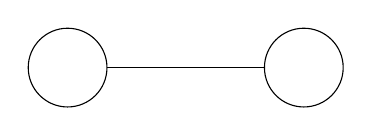
\begin{tikzpicture}
        \draw (1,1) circle (0.5 cm);
        \draw (4,1) circle (0.5 cm);
        \draw (1.5,1) -- (3.5,1); 
    \end{tikzpicture}
    \caption{$S=2^3$}
    \end{subfigure}
    ~ 
    \begin{subfigure}[b]{0.45\textwidth}
    \centering
    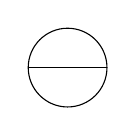
\begin{tikzpicture}
        \draw (1,1) circle (0.5 cm);
        \draw (0.5,1) -- (1.5,1); 
    \end{tikzpicture}
    \caption{$S=2\times 3!$}
    \end{subfigure}
    \caption{Diagrams with $P=3$, $V=2$, $E=0$.}
\label{p3v2e0}
\end{figure}
\begin{figure}
    \centering
                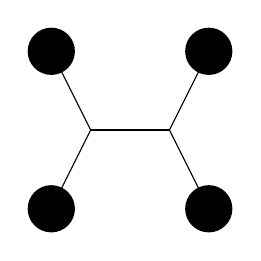
\begin{tikzpicture}
                \fill[black] (1,1) circle (0.3 cm);
                 \fill[black] (-1,1) circle (0.3 cm);
                 \fill[black] (-1,-1) circle (0.3cm);
                 \fill[black] (1,-1) circle (0.3 cm);
                 \draw (-0.5,0) -- (0.5,0);
                 \draw (-1,1) -- (-0.5,0);
                 \draw (1,1) -- (0.5,0);
                 \draw (-1,-1) -- (-0.5,0);
                 \draw (1,-1) -- (0.5,0);
            \end{tikzpicture}
    \caption{Diagram with $P=5$, $V=2$, $E=4$, and $S=2^3$.}
    \label{tree_diagramJ}
\end{figure}


\section{The path integral as the sum of connected diagrams}
Diagrams we dealt so far are all connected:  every two points can be connected by the trace of, say, a pen, continuously. However $Z(J)$ must include also other contributions arising from more general diagrams. The most general diagram $D$ is composed of the product of connected diagrams $C_I$
\begin{equation}
    D=\prod_{I}C_I^{n_I}
\end{equation}
where $C_I$ is the $I$-th connected diagram (with its symmetry factor included) and $n_I$ is the number of $C_I$'s present in $D$. However, since exchanges of propagators and vertices among different connected diagrams can result in the same diagrams, we must include an additional symmetry factor $S_D$. The exchanges that can leave the diagram unchanged are those performed between different but identical connected diagrams $C_I$. Since there are $n_I$ $C_I$'s in $D$, we can conclude that $S_D=\prod_I n_I!$, so that a general diagram reads
\begin{equation}
    D=\prod_{I}\frac{1}{n_I!}C_I^{n_I}
\end{equation}
Equation (\ref{Z_1}) tell us that $Z(J)$ is proportional to the sum over diagrams and, since diagrams are labeled by $n_I$, then
\begin{equation}
\begin{aligned}
        Z_1(J)\propto&\sum_{\{n_I\}}D\\=&\sum_{\{n_I\}}\prod_{I}\frac{1}{n_I!}C_I^{n_I}\\
        =&\sum_{n_1,n_2\dots}\frac{1}{n_1!}C_1^{n_1}\frac{1}{n_2!}C_2^{n_2}\dots\\
        =&\prod_I\sum_{n_I=0}^\infty\frac{1}{n_I!}C_I^{n_I}\\
        =&\prod_I\exp(C_I)\\
        =&\exp\sum_IC_I.
\end{aligned}
\end{equation}
A remarkable result, indicating that $Z_1(J)$ is proportional to the exponential of the sum of connected diagrams. This readily gives us a normalization criterion: if we wish $Z_1(0)=1$ we must omit \textit{vacuum diagrams} from the sum: those with no sources. With this convention we pretend vacuum diagrams don't even exist, we simply don't count them. Then, the sum of connected diagrams with no sources equals zero. We write
\begin{equation}
    Z_1(J)=\exp [iW_1(J)]
\end{equation}
where
\begin{equation}
    iW_1(J)=\sum_{I\neq\{0\}}C_I
\end{equation}
is the sum of connected diagrams omitting vacuum diagrams.\\
\section{Dealing with counterterms}
\subsection{Tadpoles}
So far we have been ignoring the other terms in the interaction Lagrangian. We analyze the consequences this leads to. The vacuum expectation value of the field is
\begin{equation}
\begin{aligned}
        \vev{\phi(x)}=&\frac{1}{i}\fdv{J(x)}Z_1(J)\eval_{J=0}\\
        =&\fdv{J(x)}W_1(J)\eval_{J=0}
\end{aligned}
\label{1Pcorrelation}
\end{equation}
In the last equality, the functional derivative removes a source from the sum of diagrams, and then, when we evaluate the derivative at $J=0$, we are left only with the diagrams that had a single source, but now have this source removed. One of these diagrams is the one shown in Figure (\ref{gJ}) with its source removed, adding the others:
\begin{equation}
    \begin{aligned}
        \vev{\phi(x)}&=
        \begin{gathered}
        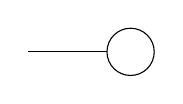
\begin{tikzpicture}
        \draw (0,0) -- (1,0);
        \draw (1.3,0) circle [radius=0.3cm];
        \end{tikzpicture}
        \end{gathered}+
        \begin{gathered}
        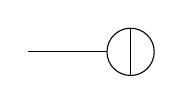
\begin{tikzpicture}
        \draw (0,0) -- (1,0);
        \draw (1.3,0) circle [radius=0.3cm];
        \draw (1.3,0.3) -- (1.3,-0.3);
        \end{tikzpicture}
        \end{gathered}+
        \begin{gathered}
        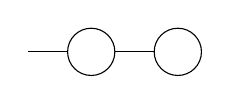
\begin{tikzpicture}
        \draw (0,0) -- (0.5,0);
        \draw (0.8,0) circle [radius=0.3cm];
        \draw (1.1,0) -- (1.6,0);
        \draw (1.9,0) circle [radius=0.3cm];
        \end{tikzpicture}
        \end{gathered}+       
        \begin{gathered}
        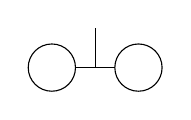
\begin{tikzpicture}
        \draw (1.35,0) -- (1.35,0.5);
        \draw (0.8,0) circle [radius=0.3cm];
        \draw (1.1,0) -- (1.6,0);
        \draw (1.9,0) circle [radius=0.3cm];
        \end{tikzpicture}
        \end{gathered}
    \\&=\frac{1}{2}iZ_gg\int\dd^4y\frac{1}{i}\Delta(x-y)\frac{1}{i}\Delta(0)+\order{g^3}.
    \end{aligned}
\end{equation}
In the last line we translated only the diagram linear in $g$. The point here is that $\vev{\phi(x)}$ is not zero, as  required by LSZ formula. This is no big news, since we are ignoring the other terms in the Lagrangian. To fix the expectation value, it's sufficient to consider the linear term $Y\phi$ from $\mathcal{L}_{\text{ct}}$, so that the interaction Lagrangian now reads
\begin{equation}
    \mathcal{L}_1=\frac{1}{3!}Z_gg\phi^3+Y\phi
\end{equation}
and (\ref{Z_1}) gets a new term
\begin{equation}
\begin{aligned}
        Z_Y(J)=&\exp\qty[\frac{1}{3!}iZ_gg\int\dd^4x\qty(\frac{1}{i}\fdv{J(x})^3+iY\int\dd^4x\, \frac{1}{i}\fdv{J(x)}]Z_0(J)\\
        =&\exp\qty[iY\int\dd^4x\, \frac{1}{i}\fdv{J(x)}]Z_1(J)\\
        =&\sum_{X=0}^\infty\frac{1}{X!}\qty[iY\int\dd^4x\, \frac{1}{i}\fdv{J(x)}]^XZ_1(J).
\end{aligned}
\label{ZY}
\end{equation}
This gives us a new series and introduce a new vertex to our diagrams: those corresponding to $iY\int\dd^4y$. The diagrams for the $X=0$ terms are all the previous diagrams we have been dealing so far. Since, for $P=2$ and $V=1$, we know the diagram for $Z_1$ linear in $g$ is that of Figure (\ref{gJ}) we built before. Now, if we consider $X=1$ in (\ref{ZY}) we get the term linear in $g$ and in $Y$:
\begin{equation}
\begin{aligned}
   Z_Y(J)&=iY \frac{Z_gg}{2}\int\dd^4x^\prime\frac{1}{i}\fdv{J(x^\prime)}
   \int\dd^4x\,\dd^4y\Delta(0)\Delta(x-y)J(y)+\order{g^3}\\
   &= \frac{YZ_gg}{2}\int\dd^4x^\prime
   \dd^4x\,\Delta(0)\Delta(x-x^\prime)+\order{g^3}
\end{aligned}
\end{equation}
which can be represented by the following diagram
\begin{equation}
    Z_Y(J)=
    \begin{gathered}
        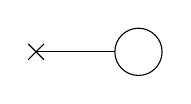
\begin{tikzpicture}
        \draw (0,0) -- (1,0);
        \draw (-0.1,-0.1) -- (0.1,0.1);
        \draw (-0.1,0.1) -- (0.1,-0.1);
        \draw (1.3,0) circle [radius=0.3cm];
        \end{tikzpicture}
        \end{gathered}
        \label{tadpole}
\end{equation}
where the line abruptly ending in a ``x" corresponds to our new vertex $iY\int\dd^4 y$. Other examples of connected diagrams with vertices from the linear counterterm are shown in Figure (\ref{diagramaX}).\\

\begin{figure}[h]
    \begin{subfigure}[]{0.2\textwidth}
    \centering
    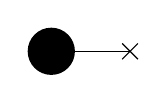
\begin{tikzpicture}
     \fill [black] (0,0) circle (0.3 cm);
    \draw (0,0) -- (1,0);
    \draw (0.9,-0.1) -- (1.1, 0.1);
    \draw (0.9,0.1) -- (1.1, -0.1);
    \end{tikzpicture}
%    \caption{$S=1$}
    \end{subfigure}
    ~ 
    \begin{subfigure}[]{0.3\textwidth}
    \centering
    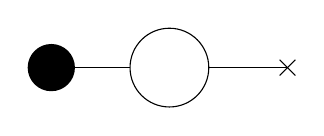
\begin{tikzpicture}
     \fill [black] (0,0) circle (0.3 cm);
    \draw (0,0) -- (1,0);
    \draw (1.5,0) circle (0.5 cm);
    \draw (2,0) -- (3,0);
    \draw (2.9,-0.1) -- (3.1, 0.1);
    \draw (2.9,0.1) -- (3.1, -0.1);
    \end{tikzpicture}
%    \caption{$S=2$}
        \end{subfigure}
    ~
    \begin{subfigure}[]{0.2\textwidth}
    \centering
    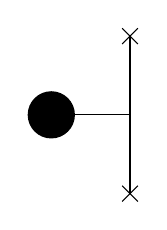
\begin{tikzpicture}
     \fill [black] (0,0) circle (0.3 cm);
    \draw (0,0) -- (1,0);
    \draw (1,-1) -- (1,1);
    \draw (0.9,-1.1) -- (1.1, -0.9);
    \draw (0.9,-0.9) -- (1.1, -1.1);
    \draw (0.9,1.1) -- (1.1, 0.9);
    \draw (0.9,0.9) -- (1.1, 1.1);
    \end{tikzpicture}
%    \caption{$S=2$}
    \end{subfigure}
    ~
    \begin{subfigure}[]{0.2\textwidth}
    \centering
    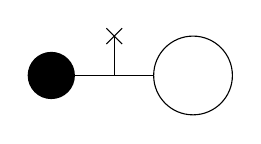
\begin{tikzpicture}
     \fill [black] (0,0) circle (0.3 cm);
    \draw (0,0) -- (1.3,0);
    \draw (1.8,0) circle (0.5 cm);
    \draw (0.8,0) -- (0.8,0.5);
    \draw (0.7,0.4) -- (0.9,0.6);
    \draw (0.7,0.6) -- (0.9,0.4);
    \end{tikzpicture}
%    \caption{$S=2$}
    \end{subfigure}
    \caption{Diagrams for (\ref{ZY}) with $E=1$, $X\geq1$}
\label{diagramaX}
\end{figure}

The same reasoning we did previously tells us that $Z_Y(J)$ equals the exponential of the sum of connected diagrams and, again, we omit vacuum diagrams (such as (\ref{tadpole})) to ensure normalization. When computing the VEV of (\ref{1Pcorrelation}), we again find it equal the sum of single source diagrams, with the sources removed. The difference now is that we include the diagrams with $X\neq 0$, such as the ones in Figure (\ref{diagramaX}). We assert that $Y=\order{g}$ and $Z_g=1+\order{g^2}$ \cite{srednicki2007quantum}, so, up to $\order{g}$, we consider $Z_g=1$ and the correlation reads
\begin{equation}
\begin{aligned}
   \vev{\phi(x)}&=
   \begin{gathered}
    \begin{tikzpicture}
    \draw (0,0) -- (1,0);
    \draw (0.9,-0.1) -- (1.1, 0.1);
    \draw (0.9,0.1) -- (1.1, -0.1);
    \end{tikzpicture}
   \end{gathered}+
   \begin{gathered}
        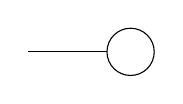
\begin{tikzpicture}
        \draw (0,0) -- (1,0);
        \draw (1.3,0) circle [radius=0.3cm];
        \end{tikzpicture}
    \end{gathered}+\order{g^3}\\
   &=\qty(iY+\frac{1}{2}i g\frac{1}{i}\Delta(0))\int\dd^4y\frac{1}{i}\Delta(x-y)+\order{g^3}.
\end{aligned}
\end{equation}
Therefore, to attain the LSZ condition, we need
\begin{equation}
    Y=\frac{1}{2}ig\Delta(0)+\order{g^3}
    \label{1pcoorelation_X}
\end{equation}
so that $\vev{\phi(x)}=0$. Being present in the Lagrangian, we know that $Y$ must be real so 
\begin{equation}
    \Delta(0)=\int\frac{\dd^4k}{(2\pi)^4}\frac{1}{k^2+m^2-i\epsilon}
\end{equation}
must be purely imaginary. The problem  is that this integral diverges, so we need to find a way to implement an ultraviolet cutoff. This cutoff is subtly implemented by considering 
\begin{equation}
    \Delta(x-y)=\int\frac{\dd^4k}{(2\pi)^4}\frac{e^{ik(x-y)}}{k^2+m^2-i\epsilon}\qty[\frac{\Lambda^2}{k^2+\Lambda^2-i\epsilon}]^2
\end{equation}
This way $\Delta(0)=i\Lambda^2/(16\pi^2)$, and we are in the position to take $\Lambda\to\infty$, making $Y\to\infty$ while $\vev{\phi(x)}=0$ \cite{srednicki2007quantum}. If we wish to calculate (\ref{1pcoorelation_X}) to higher order in $g$ we must consider the other diagrams of equation (\ref{1Pcorrelation}) and of Figure (\ref{diagramaX}).

Result (\ref{1pcoorelation_X}) indicates that the sum of diagrams of a single source, with that source removed, equals zero when considering the linear counterterm. The remarkable statement now is that if we replace that single source that gets removed by any other sub-diagram, the result still holds, the sum still vanishes. This is because if we replace the single source by the sub-diagram whose translation in terms of sources, propagators and vertices reads $\text{sub(x)}$, then the complete diagram, with a source replaced by $\text{sub(x)}$ reads $\int \dd^4x\,\text{sub(x)}\,\text{main}(x)$, where $\text{main}(x)$ is the sum of diagrams with a single source with that source removed, i.e. $\vev{\phi(x)}=0$. Thus $\int\dd^4x\,\text{sub(x)}\vev{\phi(x)}=0$. The diagrams responsible for this fact are those introduced by the linear counterterm. Diagrams cancelled with the linear counterterms are called \textit{tadpoles}. They are the ones that, when a single line is cut, leaves the diagram divided into two parts, one of which has no sources. Since they cancel with linear counterterms, we take as convention to simply ignore linear counterterms and the tadpoles altogether. \\
\subsection{Other counterterms}
We now focus on the remaining counterterms $-\frac{1}{2}(Z_\phi -1)\partial_\mu\phi\partial^\mu\phi-\frac{1}{2}(Z_m-1)m^2\phi^2$. We rename $A=Z_\phi-1$ and $B=Z_m-1$ (both of the order of $\order{g^2}$) so that the path integral reads
\begin{equation}
    Z(J)=\exp{-\frac{i}{2}\int\dd^4x\,\qty[A\partial^\mu\qty(\frac{1}{i}\fdv{j(x)})\partial_\mu\qty(\frac{1}{i}\fdv{J(x)})+\frac{1}{2}Bm^2\qty(\frac{1}{i}\fdv{J(x)})^2]}Z_Y.
\end{equation}
Integration by parts allows us to write
\begin{equation}
    Z(J)=\exp[-\frac{i}{2}\int\dd^4x\qty(\frac{1}{i}\fdv{J(x)})\qty(-A\partial^2+Bm^2)\qty(\frac{1}{i}\fdv{J(x)})]Z_Y
\end{equation}
This gives rise to a new vertex where two lines meet, for which we associate $-i\int\dd^4x(-A\partial^2+Bm^2)$. Since the lowest of these diagrams are already of the order of $g^2$, we won't be dealing with them. The diagrams we will be considering for the sum of connected diagrams $iW(J)$, thus, are the ones with or more sources, and we will ignore tadpoles and the ones arising from the linear counterterm. They are shown below, up to $g^4$. 
\begin{equation}
    \begin{aligned}
    iW(J)&=
       \begin{gathered}
            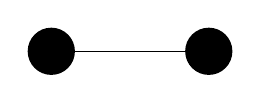
\begin{tikzpicture}
                \draw (0,0) -- (2,0);
                \fill [black] (0,0) circle (0.3 cm);
                \fill [black] (2,0) circle (0.3 cm);
            \end{tikzpicture}
       \end{gathered}
       +\begin{gathered}
            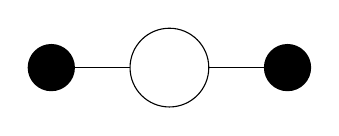
\begin{tikzpicture}
                \fill [black] (0,0) circle (0.3 cm);
                \draw (0,0) -- (1,0);
                \draw (1.5,0) circle (0.5 cm);
                \draw (2,0) -- (3,0);
                \fill [black] (3,0) circle (0.3 cm);
            \end{tikzpicture}
       \end{gathered}+
       \begin{gathered}
            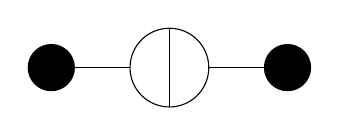
\begin{tikzpicture}
                \fill [black] (0,0) circle (0.3 cm);
                \draw (0,0) -- (1,0);
                \draw (1.5,0) circle (0.5 cm);
                \draw (2,0) -- (3,0);
                \fill [black] (3,0) circle (0.3 cm);
                \draw (1.5,0.5)--(1.5,-0.5);
            \end{tikzpicture}
       \end{gathered}\\
       &+\begin{gathered}
            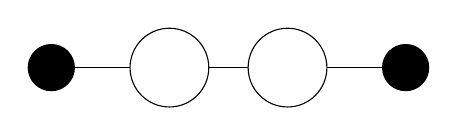
\begin{tikzpicture}
                \fill [black] (0,0) circle (0.3 cm);
                \draw (0,0) -- (1,0);
                \draw (1.5,0) circle (0.5 cm);
                \draw (2,0) -- (2.5,0);
                \draw (3,0) circle (0.5 cm);
                \draw (3.5,0) -- (4.5,0);
                \fill [black] (4.5,0) circle (0.3 cm);
            \end{tikzpicture}
       \end{gathered}+
       \begin{gathered}
            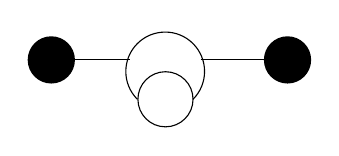
\begin{tikzpicture}
                \fill [black] (0,0) circle (0.3 cm);
                \draw (0,0) -- (1,0);
                \draw (1.8,-0.5) arc (-45:225:0.5);
                \draw (1.895,0) -- (3,0);
                \fill [black] (3,0) circle (0.3 cm);
                \draw (1.45,-0.5) circle (0.35);
            \end{tikzpicture}
       \end{gathered}\\
       &+
       \begin{gathered}
            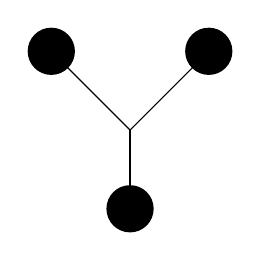
\begin{tikzpicture}
                 \fill[black] (1,1) circle (0.3 cm);
                 \fill[black] (-1,1) circle (0.3 cm);
                 \fill[black] (0,-1) circle (0.3 cm);
                 \draw (0,0) -- (1,1);
                 \draw (0,0) -- (-1,1);
                 \draw (0,0) -- (0,-1);
            \end{tikzpicture}
       \end{gathered}+
       \begin{gathered}
            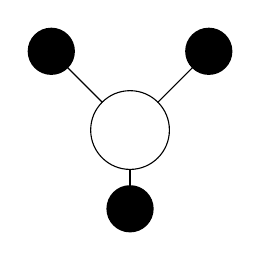
\begin{tikzpicture}
                 \fill[black] (1,1) circle (0.3 cm);
                 \fill[black] (-1,1) circle (0.3 cm);
                 \fill[black] (0,-1) circle (0.3 cm);
                 \draw (0.35,0.35) -- (1,1);
                 \draw (-0.35,0.35) -- (-1,1);
                 \draw (0,-0.5) -- (0,-1);
                 \draw (0,0) circle (0.5 cm);
            \end{tikzpicture}
       \end{gathered}+
       \begin{gathered}
            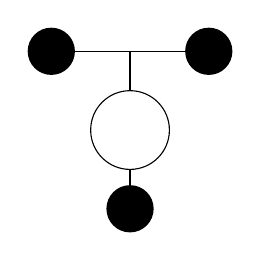
\begin{tikzpicture}
                \fill[black] (1,1) circle (0.3 cm);
                 \fill[black] (-1,1) circle (0.3 cm);
                 \fill[black] (0,-1) circle (0.3 cm);
                 \draw (-1,1) -- (1,1);
                 \draw (0,1) -- (0,0.5);
                 \draw (0,-0.5) -- (0,-1);
                 \draw (0,0) circle (0.5 cm);
            \end{tikzpicture}
       \end{gathered}+
       \begin{gathered}
            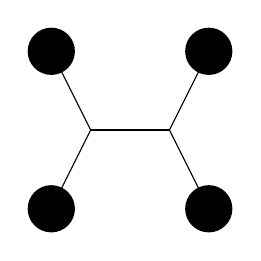
\begin{tikzpicture}
                \fill[black] (1,1) circle (0.3 cm);
                 \fill[black] (-1,1) circle (0.3 cm);
                 \fill[black] (-1,-1) circle (0.3cm);
                 \fill[black] (1,-1) circle (0.3 cm);
                 \draw (-0.5,0) -- (0.5,0);
                 \draw (-1,1) -- (-0.5,0);
                 \draw (1,1) -- (0.5,0);
                 \draw (-1,-1) -- (-0.5,0);
                 \draw (1,-1) -- (0.5,0);
            \end{tikzpicture}
       \end{gathered}\\
       &+\begin{gathered}
            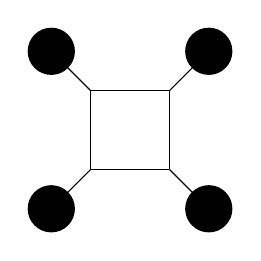
\begin{tikzpicture}
                \fill[black] (1,1) circle (0.3 cm);
                 \fill[black] (-1,1) circle (0.3 cm);
                 \fill[black] (-1,-1) circle (0.3cm);
                 \fill[black] (1,-1) circle (0.3 cm);
                 \draw (-0.5,0.5) -- (-0.5,0.5);
                 \draw (-0.5,-0.5) -- (-0.5,0.5);
                 \draw (-0.5,-0.5) -- (0.5,-0.5);
                 \draw (-0.5,0.5) -- (0.5,0.5);
                 \draw (0.5,0.5) -- (0.5,-0.5);
                 \draw (-1,1) -- (-0.5,0.5);
                 \draw (1,1) -- (0.5,0.5);
                 \draw (-1,-1) -- (-0.5,-0.5);
                 \draw (1,-1) -- (0.5,-0.5);
            \end{tikzpicture}
       \end{gathered}+
        \begin{gathered}
            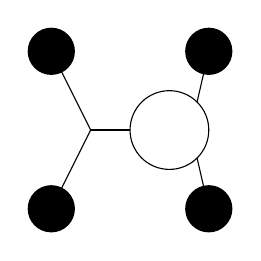
\begin{tikzpicture}
                \fill[black] (1,1) circle (0.3 cm);
                 \fill[black] (-1,1) circle (0.3 cm);
                 \fill[black] (-1,-1) circle (0.3cm);
                 \fill[black] (1,-1) circle (0.3 cm);
                 \draw (0.5,0) circle (0.5 cm);
                 \draw (-0.5,0) -- (0,0);
                 \draw (-1,1) -- (-0.5,0);
                 \draw (1,1) -- (0.85,0.35);
                 \draw (-1,-1) -- (-0.5,0);
                 \draw (1,-1) -- (0.85,-0.35);
            \end{tikzpicture}
       \end{gathered}+
        \begin{gathered}
            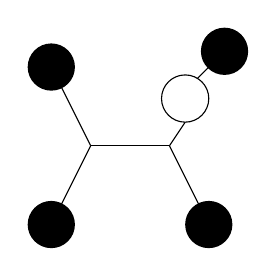
\begin{tikzpicture}
                \fill[black] (1.2,1.2) circle (0.3 cm);
                 \fill[black] (-1,1) circle (0.3 cm);
                 \fill[black] (-1,-1) circle (0.3cm);
                 \fill[black] (1,-1) circle (0.3 cm);
                 \draw (-0.5,0) -- (0.5,0);
                 \draw (-1,1) -- (-0.5,0);
                 \draw (0.7,0.3) -- (0.5,0);
                 \draw (-1,-1) -- (-0.5,0);
                 \draw (1,-1) -- (0.5,0);
                 \draw (0.85,0.85) -- (1.2,1.2);
                 \draw (0.7,0.6) circle (0.3cm);
            \end{tikzpicture}
       \end{gathered}+
       \begin{gathered}
            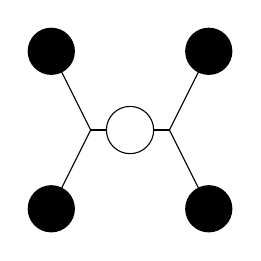
\begin{tikzpicture}
                \fill[black] (1,1) circle (0.3 cm);
                 \fill[black] (-1,1) circle (0.3 cm);
                 \fill[black] (-1,-1) circle (0.3cm);
                 \fill[black] (1,-1) circle (0.3 cm);
                 \draw (-0.5,0) -- (-0.3,0);
                 \draw (0.3,0) -- (0.5,0);
                 \draw (-1,1) -- (-0.5,0);
                 \draw (1,1) -- (0.5,0);
                 \draw (-1,-1) -- (-0.5,0);
                 \draw (1,-1) -- (0.5,0);
                 \draw (0,0) circle (0.3 cm);
            \end{tikzpicture}
       \end{gathered}+\order{g^5}
    \end{aligned}
    \label{iWphi3}
\end{equation}
\section{Feynman diagrams for $\phi^4$ theory}
For this theory, we consider the Lagrangian $\mathcal{L}=\mathcal{L}_0+\mathcal{L}_1$ where now
\begin{equation}
    \mathcal{L}_1=-\frac{1}{4!}Z_\lambda\lambda\phi^4(x)+\mathcal{L}_{\text{ct}},
\end{equation}
$\mathcal{L}_0$ and $\mathcal{L}_{\text{ct}}$ are as in (\ref{L_0}) and (\ref{L_ct}), respectively. Again, the functional integral takes the form of (\ref{interac_out_functional}). Ignoring counterterms, we have
\begin{equation}
    Z(J)=\sum_{V=0}^\infty\frac{1}{V!}\qty[\frac{iZ_\lambda\lambda}{4!}\int\dd^4x\qty(\frac{1}{i}\fdv{J(x)})^4]^V\sum_{P=0}^\infty\frac{1}{P!}\qty[\frac{i}{2}\int\dd^4x\,\dd^4y\,J(x)\Delta(x-y)J(y)]^P.
\end{equation}
The functional derivatives act on the propagators leaving $E=2P-4V$ sources remaining and an overall phase $i^{P-3V}=i^{E+V-P}$. Feynman diagrams are built according to these rules:
\begin{itemize}
    \item A vertex is where \textit{four lines} meet, and we associate $iZ_\lambda\lambda\int\dd^4x$ to it.
    \item A source is represented by a blob, and we associate $i\int\dd^4x\,J(x)$ for each one of them
    \item A line joining points $x$ and $y$ corresponds to the propagator $\frac{1}{i}\Delta(x-y)$
\end{itemize} 
The contributions to the sum of connected diagrams with $0<V\leq2$ and $0<E\leq4$ (omitting vacuum diagrams) are shown below.\\
\begin{equation}
    \begin{aligned}
    iW_1(J)&=
    \begin{gathered}
        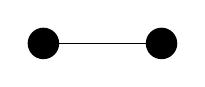
\begin{tikzpicture}
        \fill [black] (0,0) circle (0.2 cm);
        \draw (0,0) -- (1.5,0);
        \fill[black] (1.5,0) circle (0.2cm);
        \end{tikzpicture}
    \end{gathered}+
    \begin{gathered}
        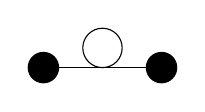
\begin{tikzpicture}
        \fill [black] (0,0) circle (0.2 cm);
        \draw (0,0) -- (1.5,0);
        \fill[black] (1.5,0) circle (0.2cm);
        \draw (0.75,0.25) circle (0.25 cm);
        \end{tikzpicture}
    \end{gathered}+
    \begin{gathered}
        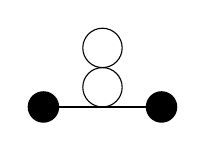
\begin{tikzpicture}
        \fill [black] (0,0) circle (0.2 cm);
        \draw (0,0) -- (1.5,0);
        \fill[black] (1.5,0) circle (0.2cm);
        \draw (0.75,0.25) circle (0.25 cm);
        \draw (0.75,0.75) circle (0.25 cm);
        \end{tikzpicture}
    \end{gathered}+
    \begin{gathered}
        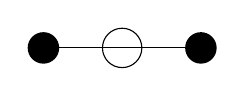
\begin{tikzpicture}
        \fill [black] (0,0) circle (0.2 cm);
        \draw (0,0) -- (2,0);
        \fill[black] (2,0) circle (0.2cm);
        \draw (1,0) circle (0.25 cm);
        \end{tikzpicture}
    \end{gathered}\\
    &+\begin{gathered}
        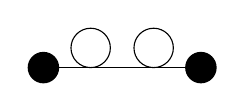
\begin{tikzpicture}
        \fill [black] (0,0) circle (0.2 cm);
        \draw (0,0) -- (2,0);
        \fill[black] (2,0) circle (0.2cm);
        \draw (0.6,0.25) circle (0.25 cm);
        \draw (1.4,0.25) circle (0.25 cm);
        \end{tikzpicture}
    \end{gathered}+
    \begin{gathered}
        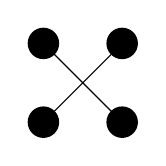
\begin{tikzpicture}
        \fill [black] (-0.5,-0.5) circle (0.2 cm);
        \fill [black] (-0.5,0.5) circle (0.2 cm);
        \fill [black] (0.5,0.5) circle (0.2 cm);
        \fill [black] (0.5,-0.5) circle (0.2 cm);
        \draw (-0.5,-0.5) -- (0.5,0.5);
        \draw (-0.5,0.5) -- (0.5,-0.5);
        \end{tikzpicture}
    \end{gathered}+
    \begin{gathered}
        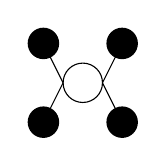
\begin{tikzpicture}
        \fill [black] (-0.5,-0.5) circle (0.2 cm);
        \fill [black] (-0.5,0.5) circle (0.2 cm);
        \fill [black] (0.5,0.5) circle (0.2 cm);
        \fill [black] (0.5,-0.5) circle (0.2 cm);
        \draw (0,0) circle (0.25 cm);
        \draw (-0.5,-0.5) -- (-0.25,0);
        \draw (-0.5,0.5) -- (-0.25,0);
        \draw (0.5,0.5) -- (0.25,0);
        \draw (0.5,-0.5) -- (0.25,0);
        \end{tikzpicture}
    \end{gathered}+
    \begin{gathered}
        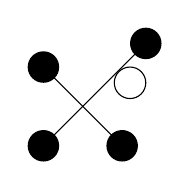
\begin{tikzpicture}
        \fill [black] (-0.5,-0.5) circle (0.2 cm);
        \fill [black] (-0.5,0.5) circle (0.2 cm);
        \fill [black] (0.8,0.8) circle (0.2 cm);
        \fill [black] (0.5,-0.5) circle (0.2 cm);
        \draw (-0.5,-0.5) -- (0.8,0.8);
        \draw (-0.5,0.5) -- (0.5,-0.5);
        \draw (0.6,0.3) circle (0.2 cm);
        \end{tikzpicture}
    \end{gathered}
    +\order{\lambda^3}
    \end{aligned}
    \label{W_phi4}
\end{equation}

We analyze the vacuum expectation value for the field in $\phi^4$ to check the consistency with the requirement from the LSZ formula:
\begin{equation}
    \vev{\phi(x)}=\frac{1}{i}\fdv{J(x)}Z_1(J)\eval_{J=0}
    \label{vevphi4}
\end{equation}
since $Z_1(J)=\exp[iW_1]$, (\ref{vevphi4}) is
\begin{equation}
    \vev{\phi(x)}=\fdv{J(x)}W_1\eval_{J=0}
\end{equation}
the sum of diagrams with a single source, with that source removed. As (\ref{W_phi4}) tells us, there are no diagrams of a single source contributing, so $\vev{\phi(x)}$ is precisely zero, and we are in good terms with the requirements from LSZ formula without having to introduce a linear counterterm. Ignoring also the other counterterms, we can take $iW(J)=iW_1(J)$ and $Z(J)=Z_1(J)$.


